\chapter{PN and orthogonal sequences}

There are two main goals need to be pursued for receiving higher localization accuracy.\\    
First the code which is used for the under water localization needs an auto-correlation approaching a Dirac impulse. Resulting in advantageous detection by correlation capabilities.\\
The next factor are cross-correlation properties, which should meet certain criteria for improving the separation from other sequences. Mathematically speaking, the codes need to be orthogonal to each other or at least approaching orthogonality. These will come in handy if noise, reflections and other artifacts emerge in real world scenarios.

\section{Pseudo-random codes}

There are a couple of techniques to generate PN sequences. Most of these methods use linear feedback shift registers to generate the codes by an initial condition or seed value. In this project I will concertize my research on gold codes, kasami codes and the basic m-sequences which are used for generating gold codes. These types are all based on linear shift registers.\\
M-sequences are defined as binary PN codes, which are generated by linear shift registers with feedback. The sequences are periodic, and contain an equal number of zeros and ones \cite{proakis08}. 
Maximum length sequences need to fulfill certain criteria.  First its length is defined by $N=2^n - 1$ where $n$ is the maximum degree of the generator polynomial $f(X)$ \cite{sarwate80}.
 \begin{equation}
	 \lvert u\rvert=2^n-1=N,~~~\text{from polynomial}~~h(x) \text{of degree}~~n
\end{equation}
\begin{equation}
	\dfrac{N}{gcd(N,q)=N},~~~\text{from decimation polynomials}~~\widetilde{h(x)}
\end{equation}
Second the cross-correlation between m-sequences must take three values only, which are $-1$, $-t(n)$, $t(n) - 2$. With it $t(n)$ is defined by $1+2^{\lfloor0.5(n+2)\rfloor}$ \cite{sarwate80}.
If every pair of m-sequences is a preferred pair, they form a maximal connected set and these sets have a limited carnality. Experiments from Gold and Koptizke showed that the number of such connected pairs is limited. Between degrees $$$$ \cite{gold65}. To get an m-sequence we need a primitive polynomial. 

%\fignoframe{images/lfsr}{Basic structure of an LFSR (Linear Feedback Register). \cite{proakis08}}{fig:framelessFigures}

\subsection{Gold Codes}

Because of not optimal cross-correlation properties m-sequences alone are not applicable for the project. But if these type of codes are combined their correlation qualities can change. Gold Codes are m-sequences where two of them with same length are modulo-2 summed. \cite{proakis08} \\
Recent research shows that some gold codes have high similarity to a Gaussian random variable \cite{merrifield}. 

\begin{equation}
Gold(u,v)=\{u,v,u\oplus v,u\oplus(v \ll1),\dots,u\oplus(v\ll N-1)\}
\end{equation}

%\fignoframe{images/gold}{LFSR structure of preferred generator polynomial of degree 13. \cite{merrifield}}{fig:framelessFigures}

\subsection{Kasami Codes}

Kasami sequences are constructed in the similar fashion by using m-sequences with the exception that a second sequence, which is used in the modulo sum, is formed by decimating the default m-sequence by  $2^{m/2}$ \cite{proakis08} \cite{sarwate80} \cite{peterson72}. Thus, only one generator polynomial is required.

\begin{equation}
w=u[2^{N/2}+1]=\{u_1,\dots, u_i, \dots,u_{N}|\text{take every }i\text{-th bit of u}\} 
\end{equation}
\begin{equation}
Kasami(u)=\{u,u\oplus w,u\oplus(w \ll1),\dots,u\oplus(w\ll2^{N/2}-2)\}
\end{equation}


\section{Comparison}

For the localization process by orthogonal codes certain criteria needs to be met, which were named in the first chapter. To compare the before explained code types three measures are introduced. \\ 
The first one is the peak to side-lobe ratio (PSR) \ref{eq:psr}. This measure is defined by subtracting the mean from the peak of the auto-correlation. Then this value get divided by the standard deviation of the same auto-correlation. A higher PSR value signifies a lower error between the auto correlation and the perfect Dirac resulting in better detection capability. The second one is the ratio between the auto-correlation peak and the maximum of the cross-correlation (ACR) \ref{eq:acr}. There a higher value indicates good code separation qualities. 
%The last one is the correlation coefficient showing if there are similar anchros \ref{eq:coeff}, which would be a bad indicator.

\begin{equation}
PSR=\dfrac{max\{x_{ac}\}-\overline{x_{ac}}}{\sigma_{ac}}
\label{eq:psr}
\end{equation}

\begin{equation}
ACR=\dfrac{max\{x_{ac}\}}{max\{{x_{cc}\}}}
\label{eq:acr}
\end{equation}

%\begin{equation}
%\rho(a1,a2)=\dfrac{cov\{a1,a2\}}{\sigma_{a1}\cdot\sigma_{a2}}
%\label{eq:coeff}
%\end{equation}
%\begin{figure}[h]
%	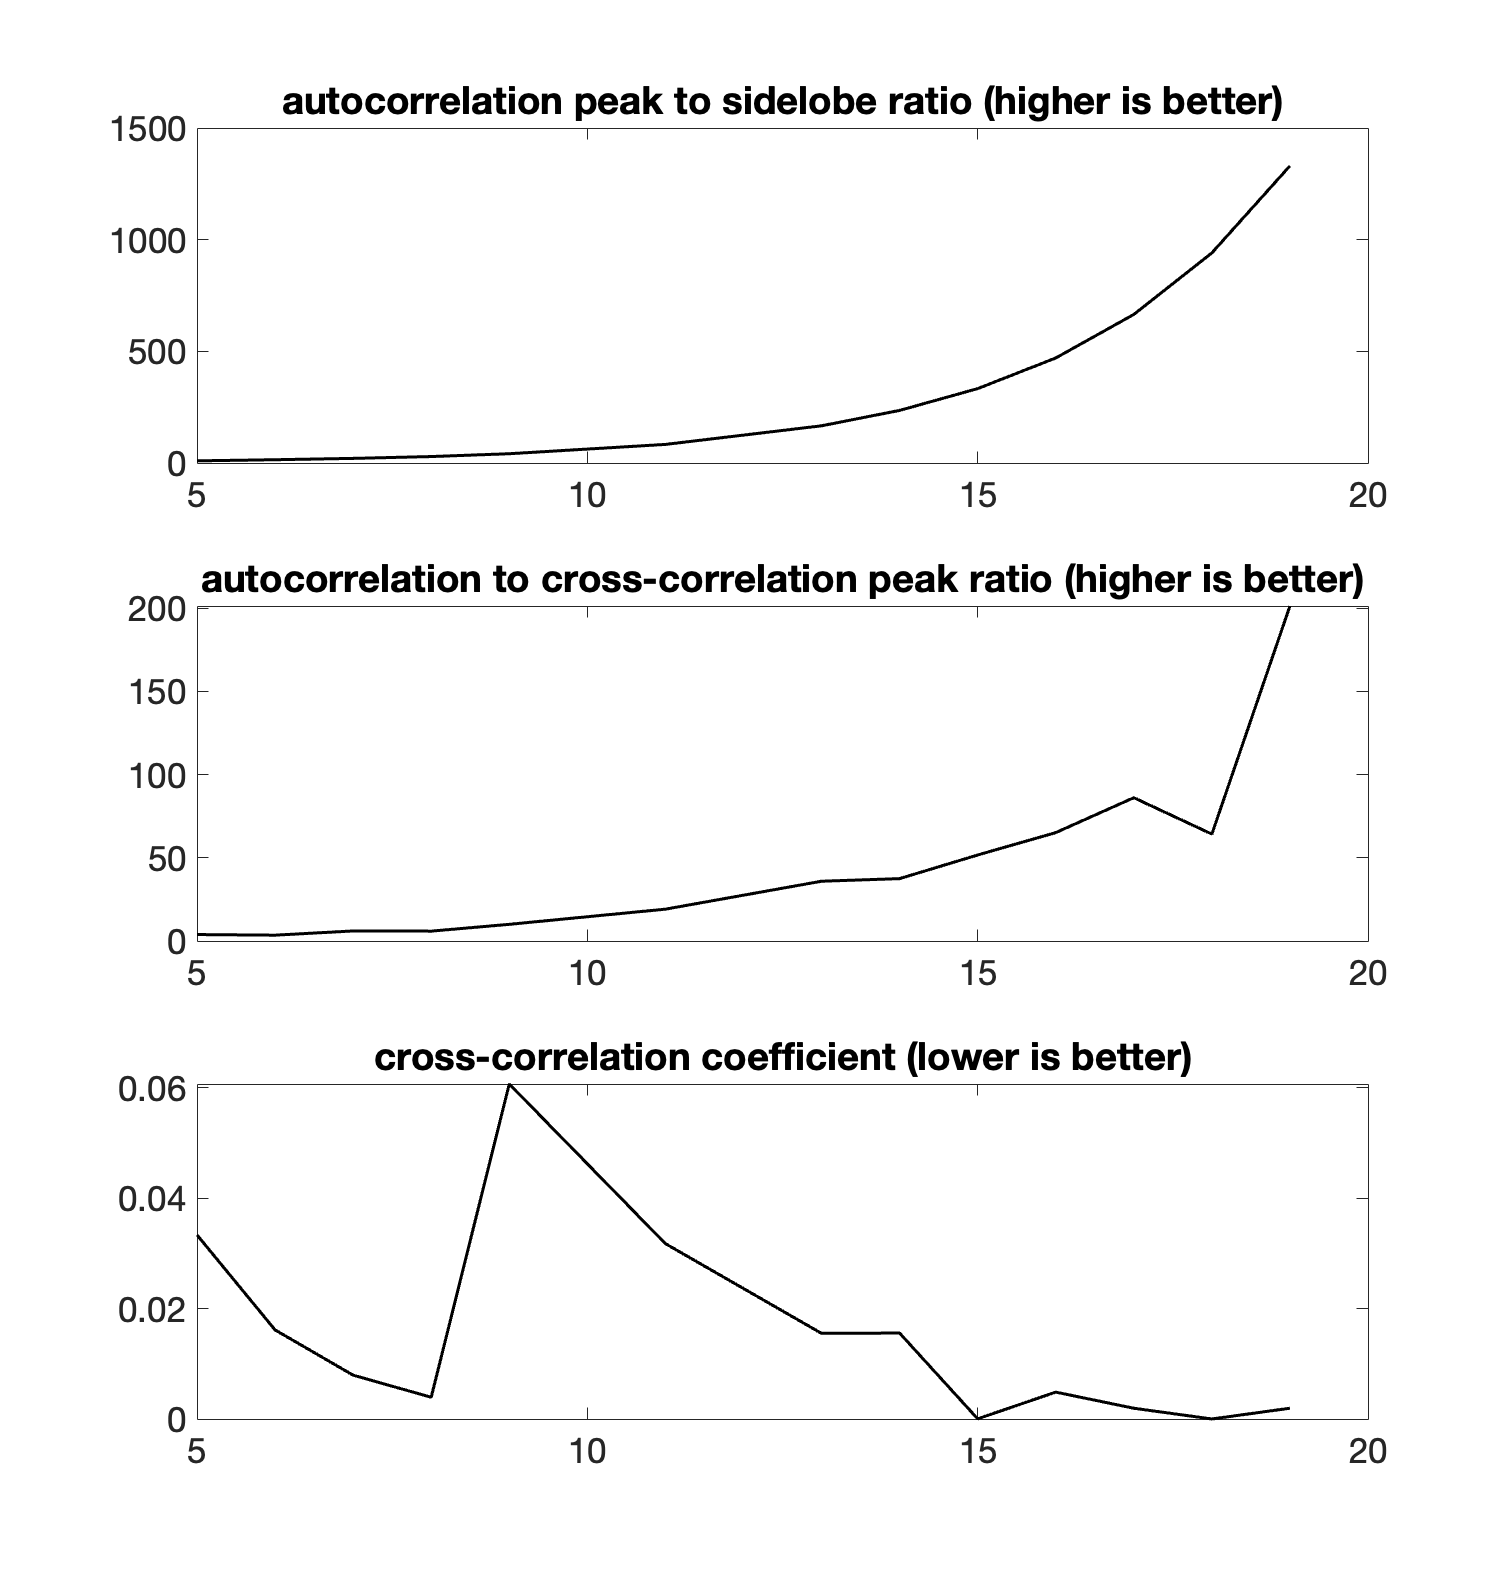
\includegraphics[width=8cm]{images/matlabplots/mseq}
%
%	\caption{Maximum Length Sequence evaluation}
%\end{figure}
%
%\begin{figure}[h]
%	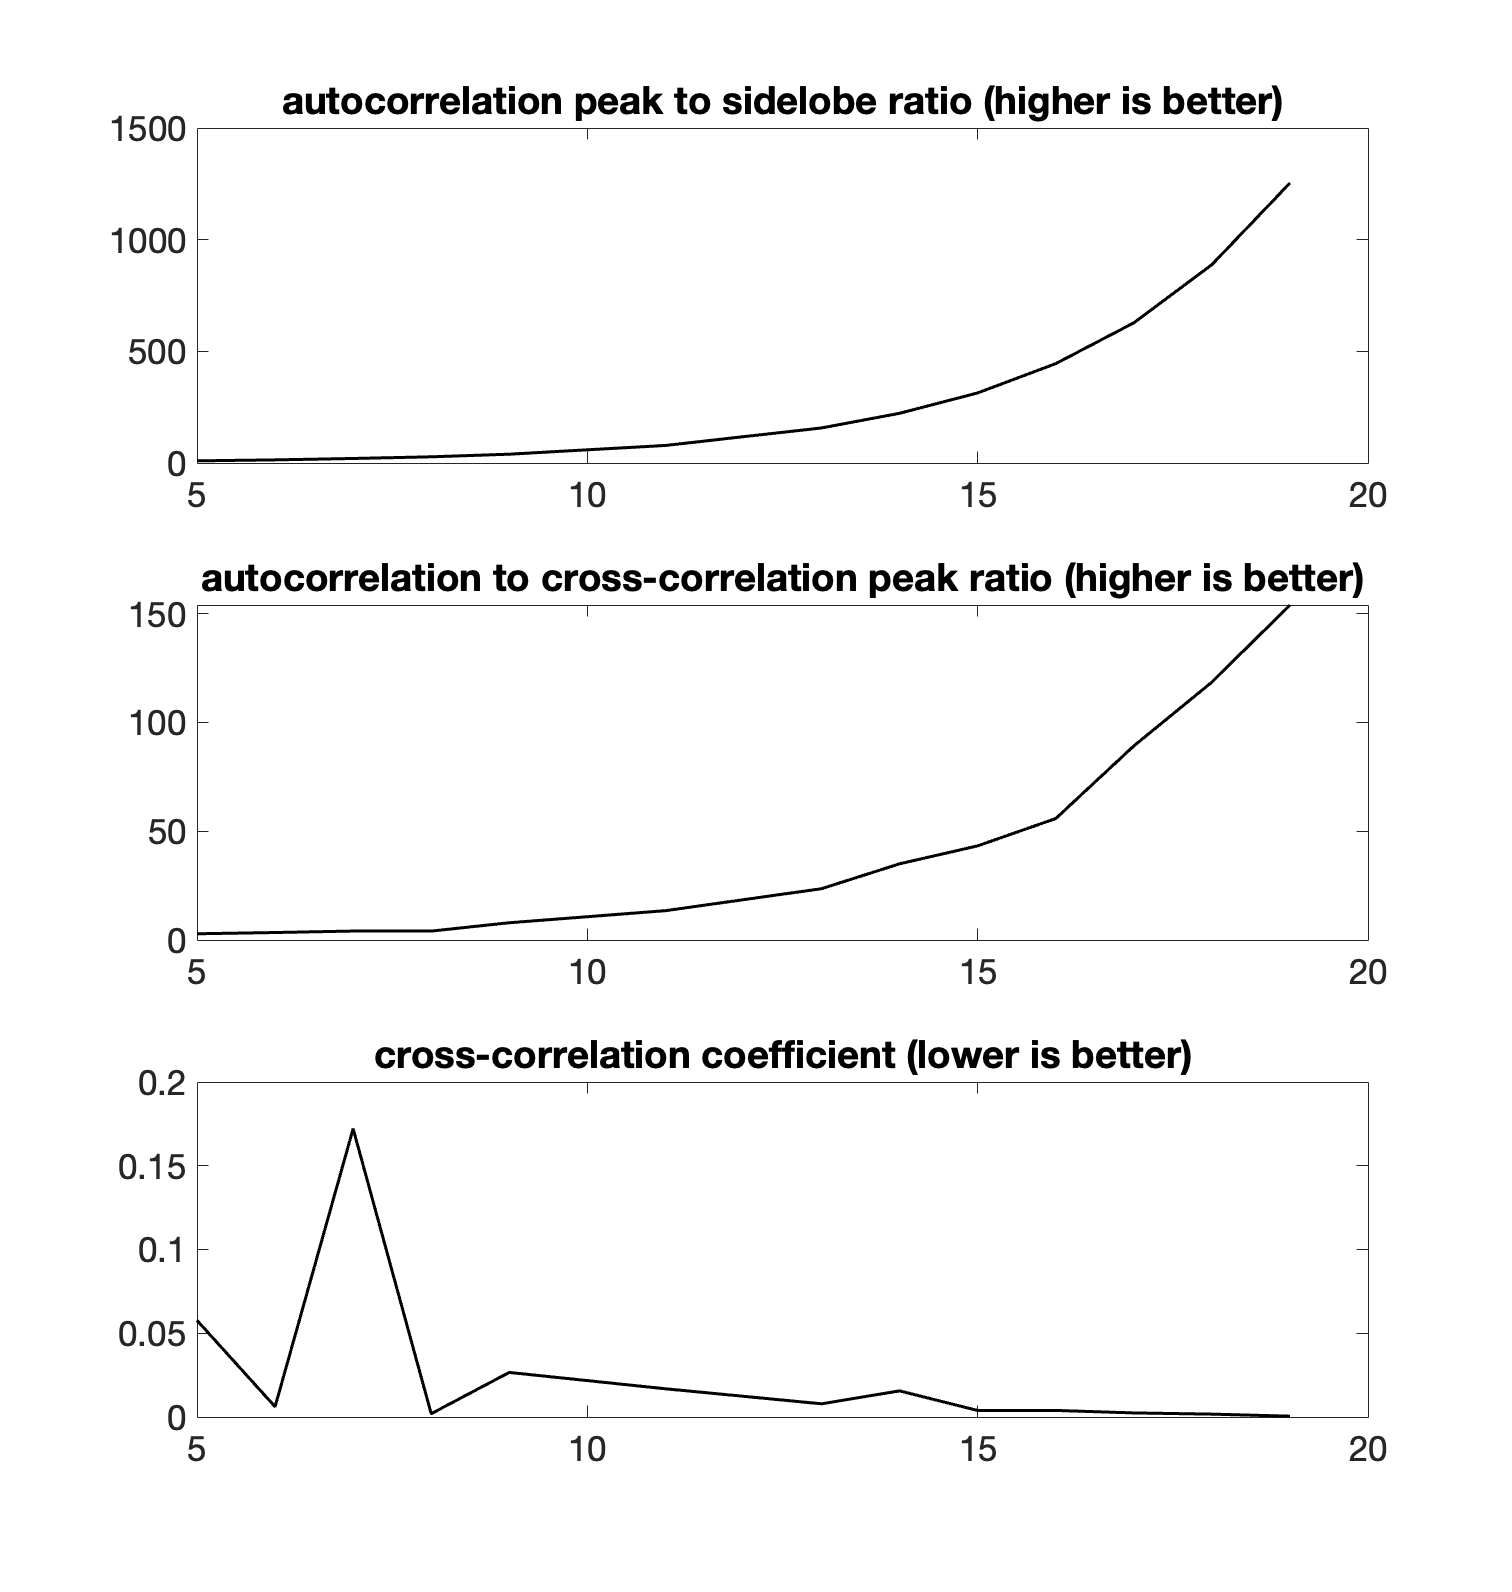
\includegraphics[width=8cm]{images/matlabplots/gold}
%
%	\caption{Gold sequence evaluation}
%\end{figure}
%
%\begin{figure}[h]
%	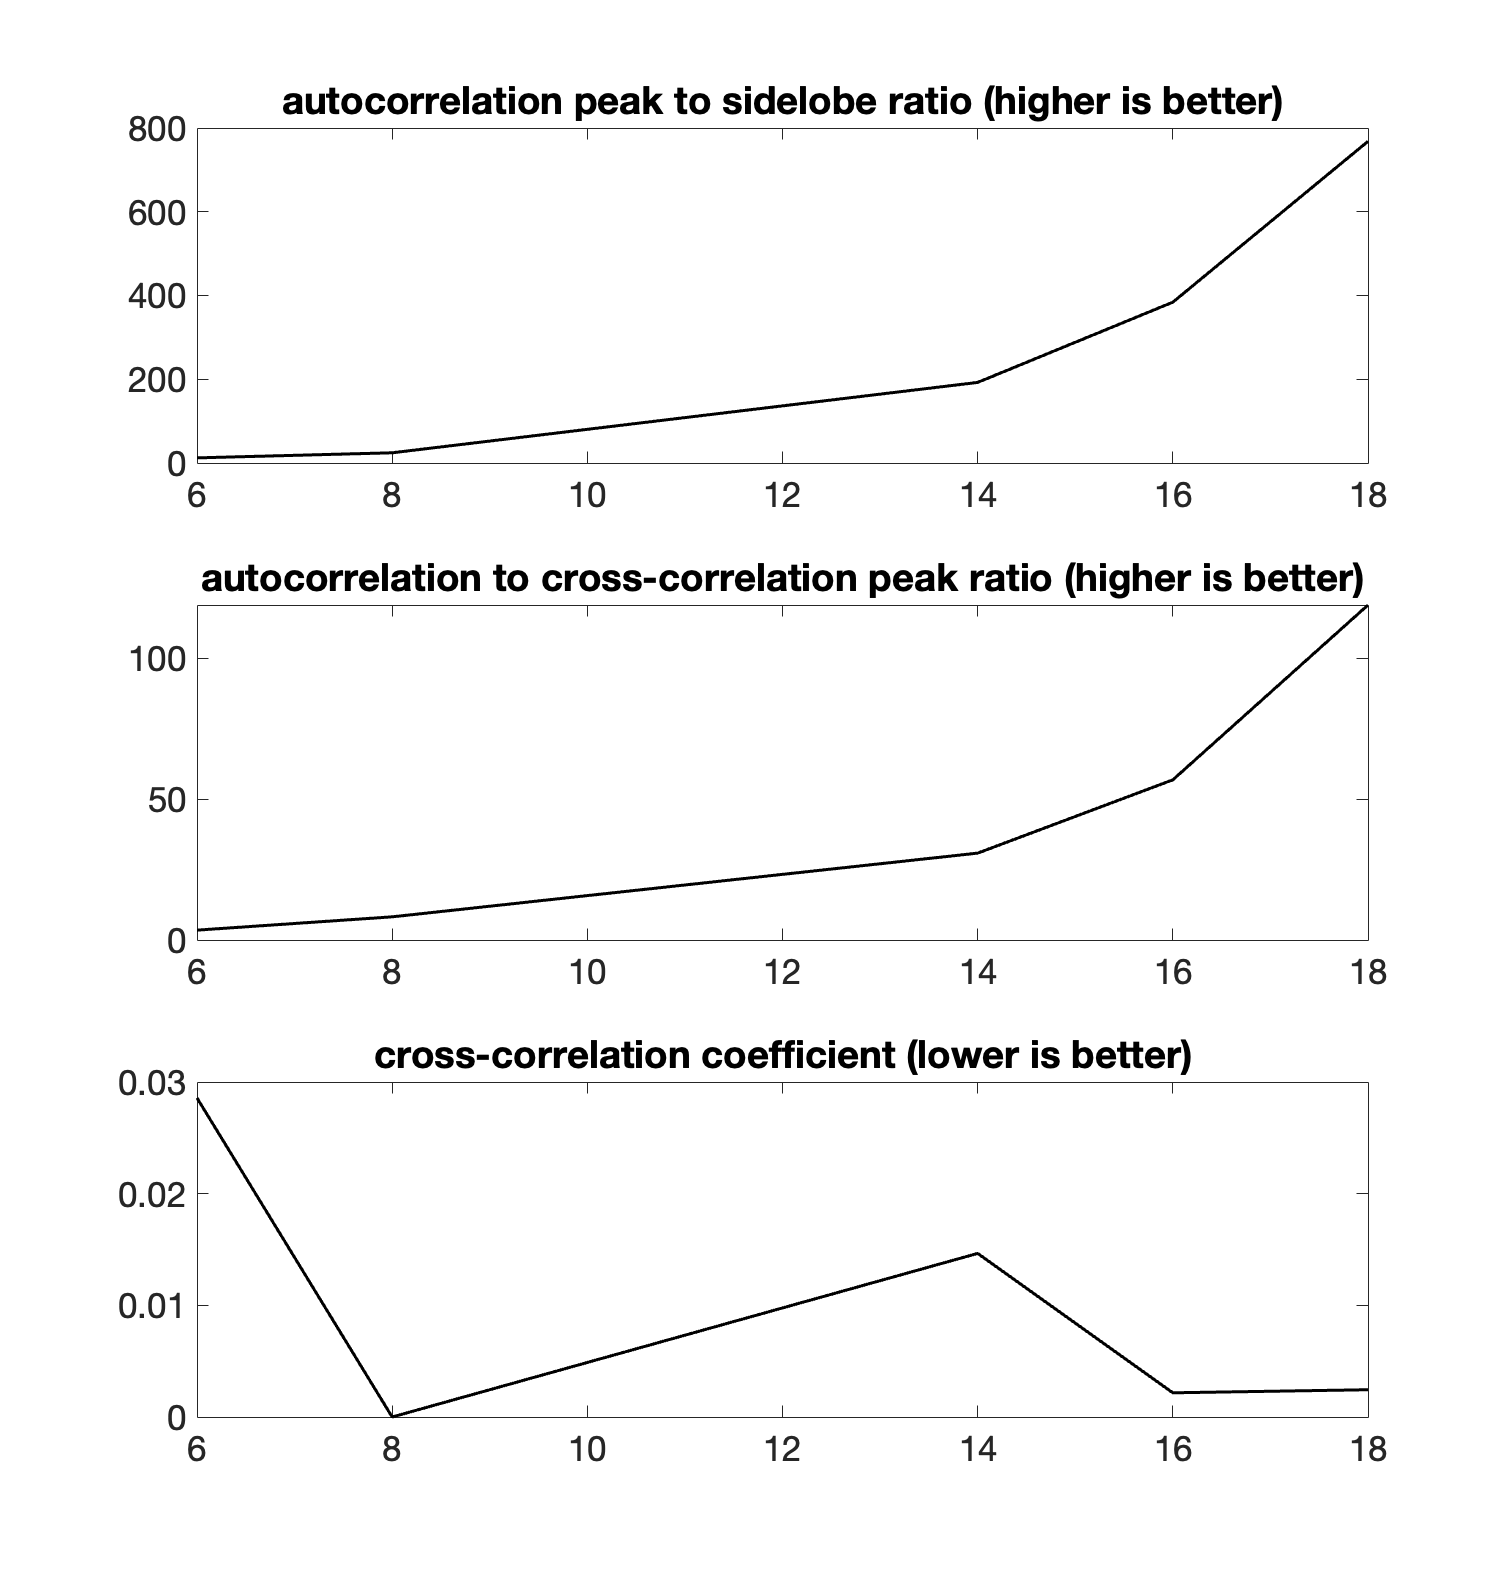
\includegraphics[width=8cm]{images/matlabplots/kasami}
%
%	\caption{Kasami sequence evaluation}
%\end{figure}
%%\fignoframe{images/matlabplots/mseq}{Basic structure of an LFSR (Linear Feedback Register). \cite{proakis08}}{fig:framelessFigures}
%%\fignoframe{images/matlabplots/gold\_10ms}{Basic structure of an LFSR (Linear Feedback Register). \cite{proakis08}}{fig:framelessFigures}
%%\fignoframe{images/matlabplots/kasami\_10ms}{Basic structure of an LFSR (Linear Feedback Register). \cite{proakis08}}{fig:framelessFigures}
%\section{Results}

From preferred polynomial all possible maximum length sequences, gold sequences and kasami sequences are generated. Then both measures are applied on the cross-correlation and auto-correlation functions of the random codes. The PSR and ACR measures are plotted against the used polynomials. Also the best case of PSR and ACR are plotted by their given correlation function.\\
Maximum length sequences hold the best auto-correlation properties in comparison to its competitors. But it shows peaks in its cross-correlation, making it a rather bad option for orthogonal separation. The kasami sequence has a way better cross-correlation but still a small peak. The clear winner are gold codes because of the good auto-correlation and very good cross-correlation properties \ref{fig:eva}. Its auto-correlations lags a bit behind its competitors but orthogonality is as much as important. 
%
%\begin{figure}[h]
%	\centering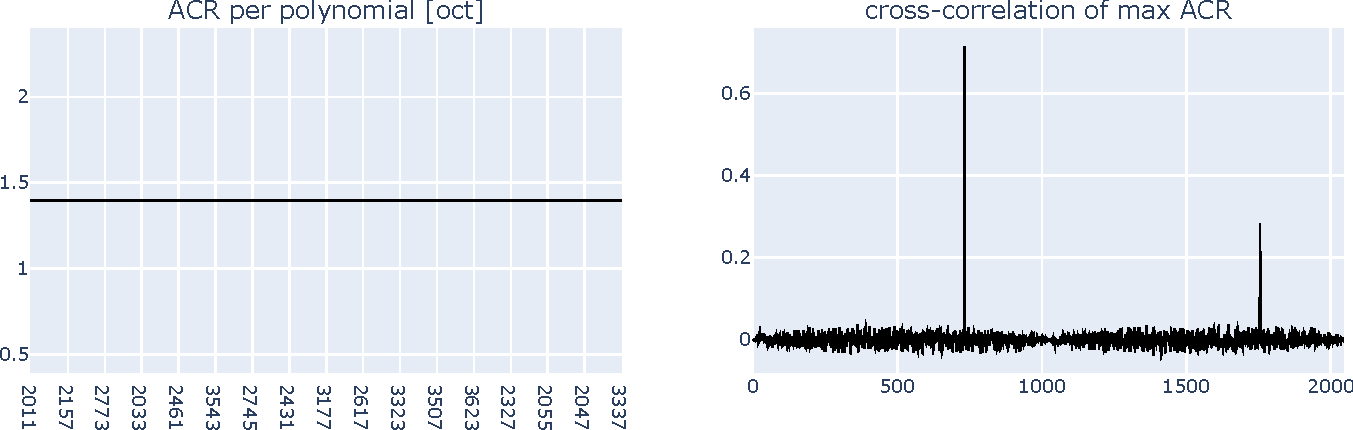
\includegraphics[width=13cm]{images/mseqevaacr}
%	
%	\caption{Evaluation of m-sequences by AC ratio}
%	\label{fig:eva}
%\end{figure}
%
%\begin{figure}[h]
%	\centering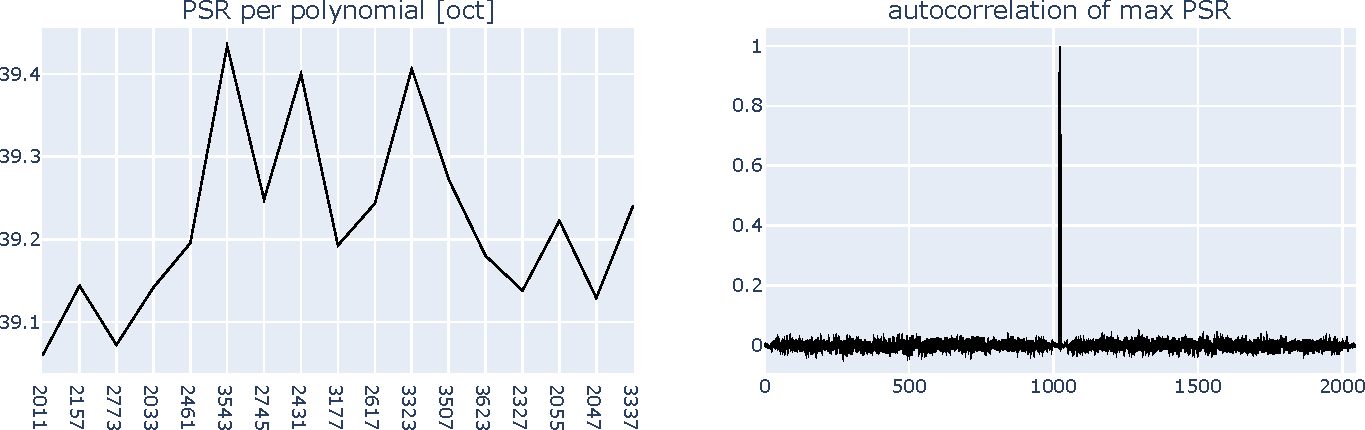
\includegraphics[width=13cm]{images/mseqevapsr}
%	
%	\caption{Evaluation of m-sequences by PS ratio}
%	\label{fig:eva}
%\end{figure}

\begin{figure}[h]
	\centering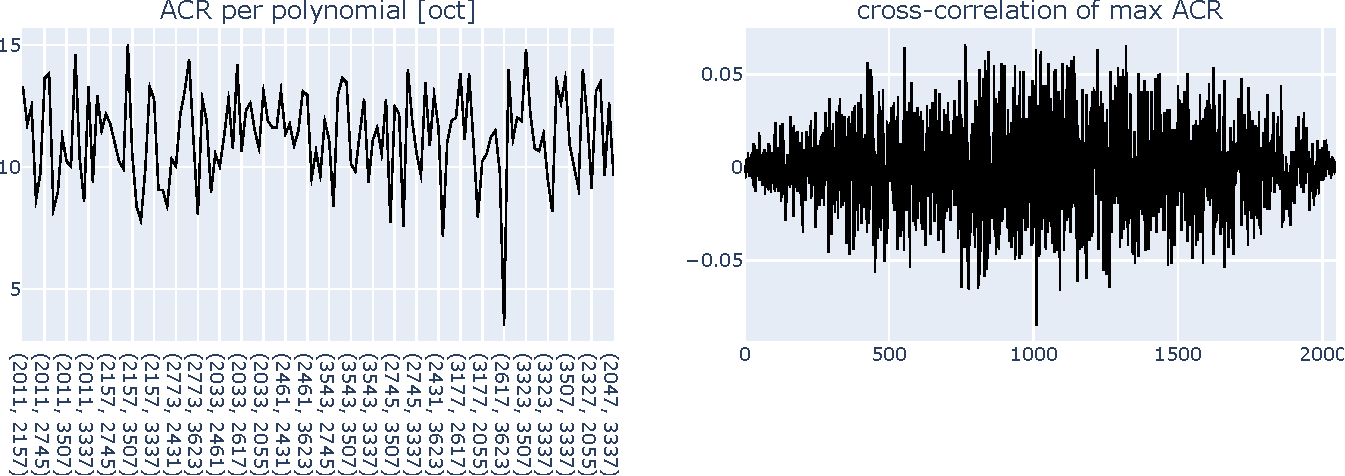
\includegraphics[width=13cm]{images/goldevaacr}
	
	\caption{Evaluation of gold sequences by AC ratio}
	\label{fig:eva}
\end{figure}

\begin{figure}[h]
	\centering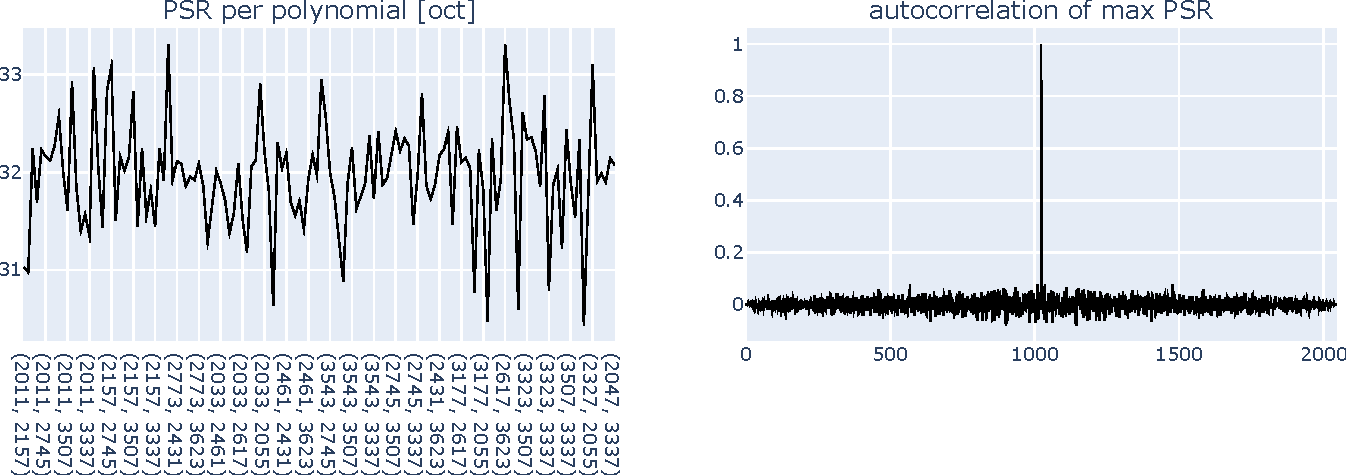
\includegraphics[width=13cm]{images/goldevapsr}
	
	\caption{Evaluation of gold sequences by PS ratio}
	\label{fig:eva}
\end{figure}

\begin{figure}[h]
	\centering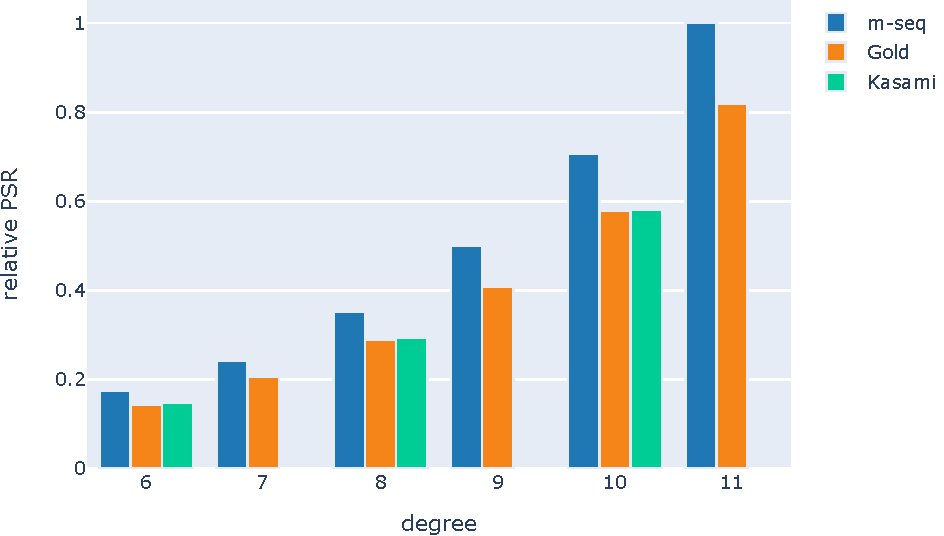
\includegraphics[width=13cm]{images/degPsrEva}
	
	\caption{Evaluation by relative PSR for degrees 6 to 11}
	\label{fig:eva}
\end{figure}

\begin{figure}[h]
	\centering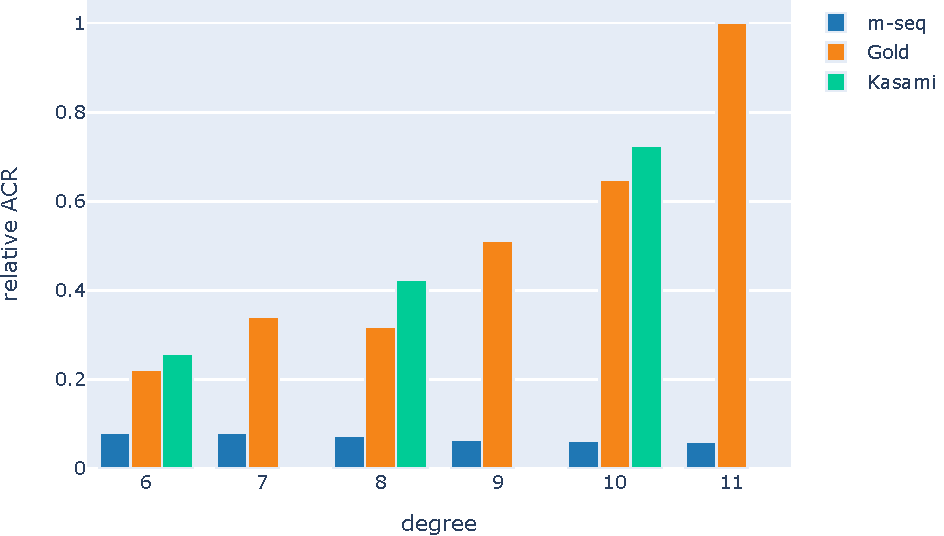
\includegraphics[width=13cm]{images/degAcrEva}
	
	\caption{Evaluation by relative ACR for degrees 6 to 11}
	\label{fig:eva}
\end{figure}
